\documentclass[preprint,12pt,aps,pra,showkeys,amsmath,amssymb,superscriptaddress,floatfix]{revtex4-2}
\usepackage[T1]{fontenc}
\usepackage[utf8]{inputenc}
\usepackage{amsmath,amssymb,amsthm,mathtools,mathrsfs}
\usepackage{microtype,booktabs,enumitem}
\usepackage{xcolor,tikz,etoolbox}
\usepackage[skins,breakable]{tcolorbox}
\usepackage{needspace}
% Keep diagram geometry independent of REVTeX preprint body spacing.
\AtBeginEnvironment{tikzpicture}{\linespread{1}\selectfont}
\usetikzlibrary{arrows.meta,positioning,calc,fit,decorations.pathreplacing}
\usepackage{graphicx}
\usepackage{hyperref}

\definecolor{MMBlue}{RGB}{0,82,155}
\definecolor{MMOrange}{RGB}{200,80,0}
\tikzset{
 mmnode/.style={draw=MMBlue,rounded corners=2pt,fill=MMBlue!4,align=left,execute at begin node={\raggedright},text width=5cm,font=\fontsize{10}{12}\selectfont,inner sep=6pt},
 mmimport/.style={mmnode,draw=black!65,fill=black!4},
 mmcandidate/.style={mmnode,draw=MMOrange,dashed,fill=MMOrange!5},
 mmrejected/.style={mmnode,draw=black,densely dotted,fill=black!8},
 mmproof/.style={->,thick,MMBlue},
 mmflow/.style={->,semithick,black!70},
 mmrepair/.style={->,dashed,thick,MMOrange},
 mmcandidatearrow/.style={->,dashed,semithick,MMOrange},
 mmnote/.style={font=\scriptsize,fill=white,inner sep=2pt,align=center}}

\usepackage[section]{placeins}
\setlength{\emergencystretch}{3em}
\setlist{itemsep=3pt,topsep=4pt}
\newtheorem{theorem}{Theorem}[section]
\newtheorem{proposition}[theorem]{Proposition}
\newtheorem{lemma}[theorem]{Lemma}
\newtheorem{corollary}[theorem]{Corollary}
\theoremstyle{definition}
\newtheorem{definition}[theorem]{Definition}
\newtheorem{example}[theorem]{Example}
\theoremstyle{remark}
\newtheorem{remark}[theorem]{Remark}
% Avoid isolated statement headings and single-line paragraph fragments.
\BeforeBeginEnvironment{theorem}{\Needspace{6\baselineskip}}
\BeforeBeginEnvironment{definition}{\Needspace{5\baselineskip}}
\BeforeBeginEnvironment{proposition}{\Needspace{5\baselineskip}}
\BeforeBeginEnvironment{lemma}{\Needspace{5\baselineskip}}
\BeforeBeginEnvironment{corollary}{\Needspace{5\baselineskip}}
\clubpenalty=5000
\widowpenalty=5000
\newcommand{\R}{\mathbb R}\newcommand{\Z}{\mathbb Z}\newcommand{\N}{\mathbb N}
\newcommand{\Pa}{\operatorname{Pa}}\newcommand{\Desc}{\operatorname{Desc}}
\newcommand{\cl}{\operatorname{cl}}\newcommand{\cost}{\operatorname{cost}}
\newcommand{\status}{\operatorname{status}}
% Faculty cards: a visual rail groups the five faculties within one agent.
% The rail has no arrowhead and does not represent a proof dependency.
\newcommand{\mmfacultybadge}[1]{%
 \node[circle,draw=MMBlue,line width=1pt,fill=white,
 minimum size=7mm,inner sep=0pt,font=\sffamily\small\bfseries,text=MMBlue]
 at ([xshift=15pt,yshift=-15pt]frame.north west) {#1};}
\newcommand{\mmfacultyrail}{%
 \draw[MMBlue!80,line width=1pt]
 ([xshift=15pt,yshift=2pt]frame.north west)--
 ([xshift=15pt,yshift=-2pt]frame.south west);}
\newtcolorbox{mmfacultybox}[2]{enhanced,breakable,
 colback=MMBlue!4,colframe=MMBlue!4,boxrule=0pt,arc=3pt,
 left=39pt,right=9pt,top=4pt,bottom=4pt,
 before skip=2pt,after skip=2pt,
 fontupper=\small\linespread{1.1}\selectfont,
 overlay unbroken={\mmfacultyrail\mmfacultybadge{#1}},
 overlay first={\mmfacultyrail\mmfacultybadge{#1}},
 overlay middle={\mmfacultyrail},overlay last={\mmfacultyrail}}
\newcommand{\mmfaculty}[3]{%
 \begin{mmfacultybox}{#1}{#2}
 {\sffamily\bfseries\color{MMBlue}#2}\par\smallskip #3
 \end{mmfacultybox}}
\newcommand{\agent}[9]{%
 \Needspace{8\baselineskip}
 \subsubsection{#1}
 \noindent\textbf{Object.} #2\par
 \noindent\textbf{Role.} #3\par\smallskip
 \mmfaculty{E}{Ego}{#4}
 \mmfaculty{M}{Memory}{#5}
 \mmfaculty{I}{Intellect}{#6}
 \mmfaculty{S}{Sense}{#7}
 \mmfaculty{A}{Action}{#8}
 \smallskip\noindent #9\par}

\usepackage{longtable,array,calc}
\providecommand{\tightlist}{\setlength{\itemsep}{2pt}\setlength{\parskip}{0pt}}
\makeatletter
\def\frontmatter@abstract@produce{\par\addvspace{\frontmatter@preabstractspace}%
\begingroup\prep@absbox\unvbox\absbox\post@absbox\endgroup
\addvspace{\frontmatter@postabstractspace}}
\makeatother
\newcommand{\field}[2]{\par\smallskip\noindent\textbf{#1.} #2\par}
\setlength{\emergencystretch}{5em}
\AtBeginEnvironment{verbatim}{\small\linespread{1.0}\selectfont}


\hypersetup{colorlinks=true,linkcolor=MMBlue,urlcolor=MMBlue,pdfauthor={Dibakar Sigdel}}

\begin{document}

\title{Irreducibility, Prime Ideals, and Coordinate Domains\\[4pt]\large An End-to-End Meta-Math Walkthrough}

\author{Dibakar Sigdel}

\affiliation{Mindverse Computing LLC, Lynnwood, WA 98087, USA}

\date{October 2026}

\begin{abstract}

A product vanishes at each point exactly when at least one factor does.
This translates a geometric split into zero divisors in the coordinate
ring. The report presents the target theorem, declared imports, a
dependency graph, five-faculty node contracts, a continuous proof, a
worked example, and a hypothesis-repair audit. It is an authored
mathematical exposition, not a deployed-agent transcript or a formal
proof-assistant certificate.

\end{abstract}\maketitle\linespread{1.12}\selectfont

\noindent\textbf{AG-04 / Algebraic Geometry / Report v1}

\section{Target and import contract}

\begin{theorem}

Let \(X\subset k^n\) be a nonempty affine algebraic set over a field
\(k\). With its Zariski subspace topology, \(X\) is irreducible if and
only if \(I(X)\) is prime, equivalently the coordinate ring
\(k[X]=k[x_1,\ldots,x_n]/I(X)\) is an integral domain. Irreducible means
not a union of two proper closed subsets. Algebraic closedness is not
needed for this statement about the actual point set and its vanishing
ideal.

\end{theorem}

\subsection{Foundations and permitted imports}

Use \(V(fg)=V(f)\cup V(g)\) over a field, the definition of the Zariski
topology, and the quotient criterion: a proper ideal \(P\) is prime iff
\(ab\in P\) implies \(a\in P\) or \(b\in P\). The quotient is a domain
precisely when this implication holds. Relative closed sets in \(X\) are
\(X\cap V(S)\) for collections \(S\) of polynomials.

\clearpage\section{Node interaction workflow}

\begin{center}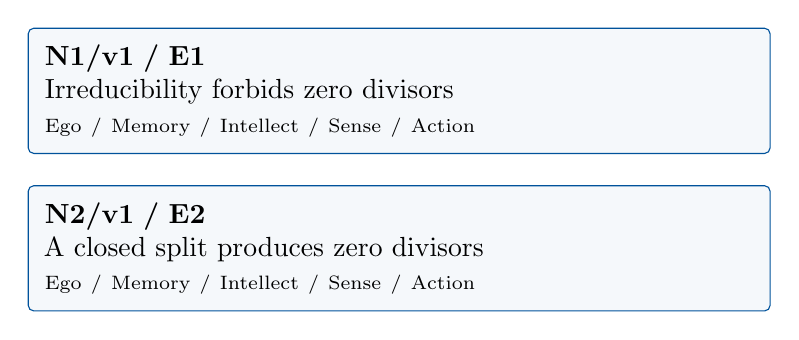
\begin{tikzpicture}[>=Stealth,x=1cm,y=1cm]

\node[mmnode,text width=9cm,minimum height=1.25cm] (N1) at (0,0.0) {\textbf{N1/v1 / E1}\\Irreducibility forbids zero divisors\\{\scriptsize Ego / Memory / Intellect / Sense / Action}};

\node[mmnode,text width=9cm,minimum height=1.25cm] (N2) at (0,-2.0) {\textbf{N2/v1 / E2}\\A closed split produces zero divisors\\{\scriptsize Ego / Memory / Intellect / Sense / Action}};

\end{tikzpicture}\end{center}

Each box is one mathematical agent containing all five faculties. Blue
arrows carry the versioned exports listed below. The layout gives a
reading order; only drawn arrows assert dependencies. Diagnostic repair
is separate from the proof DAG.

\subsection{Versioned evidence-transfer ledger}
No inter-node proof imports are needed: the nodes establish separate directions under the common theorem contract.


\begingroup\small\linespread{1.05}\selectfont

\endgroup

\clearpage\section{Agent roles and five-faculty activities}\begingroup\small\linespread{1.05}\selectfont\setlist{itemsep=1pt,topsep=2pt}

\subsection{N1/v1: Irreducibility forbids zero divisors}

\field{Object and role}{Convert a vanishing product into a two-set closed cover. \textbf{Local
obligation:} If \(X\) is irreducible then \(I(X)\) is prime.}

\field{Inputs}{Nonempty irreducible \(X\) and \(fg\in I(X)\).}

\mmfaculty{E}{Ego}{Publish E1/v1 only after establishing this obligation: If \(X\) is
irreducible then \(I(X)\) is prime.}

\mmfaculty{M}{Memory}{Nonempty irreducible \(X\) and \(fg\in I(X)\). Retain the stated
assumptions and import versions.}

\mmfaculty{I}{Intellect}{Convert a vanishing product into a two-set closed cover.}

\mmfaculty{S}{Sense}{Nonemptiness makes \(I(X)\) proper; the empty set has the unit vanishing
ideal.}

\mmfaculty{A}{Action}{Carry out activities N1.1--N1.2 below, retaining each calculation and
construction as evidence.}

\smallskip\noindent\textbf{Numbered mathematical activities}

\begin{enumerate}[label=N1.\arabic*,leftmargin=3.4em]

\item Nonemptiness gives \(1\notin I(X)\). If \(fg\in I(X)\), each point of
\(X\) lies in \(V(f)\) or \(V(g)\), because a field has no zero
divisors. Hence \(X=(X\cap V(f))\cup(X\cap V(g))\).

\item Both pieces are closed in \(X\). Irreducibility forces one to equal
\(X\), which says \(f\in I(X)\) or \(g\in I(X)\). This proves primality.

\end{enumerate}

\field{Export E1/v1}{If \(X\) is irreducible then \(I(X)\) is prime.}

\field{Acceptance gate}{Nonemptiness makes \(I(X)\) proper; the empty set has the unit vanishing
ideal.}

\field{Targeted repair}{If the empty set is included as irreducible, restore nonemptiness before
claiming a proper prime ideal. Withhold this export and recheck its
descendants after a versioned correction.}

\clearpage

\subsection{N2/v1: A closed split produces zero divisors}

\field{Object and role}{Choose one polynomial detecting a point outside each closed subset and
multiply them. \textbf{Local obligation:} If \(I(X)\) is prime then
\(X\) is irreducible, and both conditions are equivalent to \(k[X]\)
being a domain.}

\field{Inputs}{Prime \(I(X)\) and a proposed decomposition \(X=Y\cup Z\) into two
proper relatively closed subsets.}

\mmfaculty{E}{Ego}{Publish E2/v1 only after establishing this obligation: If \(I(X)\) is
prime then \(X\) is irreducible, and both conditions are equivalent to
\(k[X]\) being a domain.}

\mmfaculty{M}{Memory}{Prime \(I(X)\) and a proposed decomposition \(X=Y\cup Z\) into two
proper relatively closed subsets. Retain the stated assumptions and
import versions.}

\mmfaculty{I}{Intellect}{Choose one polynomial detecting a point outside each closed subset and
multiply them.}

\mmfaculty{S}{Sense}{A proper closed subset has a defining equation that fails somewhere on
\(X\); do not assume one equation defines the whole subset.}

\mmfaculty{A}{Action}{Carry out activities N2.1--N2.2 below, retaining each calculation and
construction as evidence.}

\smallskip\noindent\textbf{Numbered mathematical activities}

\begin{enumerate}[label=N2.\arabic*,leftmargin=3.4em]

\item Write \(Y=X\cap V(S)\) and choose \(a\in X\setminus Y\). Some \(f\in S\)
has \(f(a)\ne0\), so \(f\) vanishes on \(Y\) but is not in \(I(X)\).
Similarly choose \(g\) vanishing on \(Z\) but not on all of \(X\).

\item The product \(fg\) vanishes on \(Y\cup Z=X\), so \(fg\in I(X)\) while
neither factor belongs to it, contradicting primality. Thus a proper
split is impossible. Finally, multiplication of residue classes in
\(k[X]\) is zero exactly when the product of representatives lies in
\(I(X)\); the prime-ideal condition is exactly absence of nonzero zero
divisors, with \(1\ne0\).

\end{enumerate}

\field{Export E2/v1}{If \(I(X)\) is prime then \(X\) is irreducible, and both conditions are
equivalent to \(k[X]\) being a domain.}

\field{Acceptance gate}{A proper closed subset has a defining equation that fails somewhere on
\(X\); do not assume one equation defines the whole subset.}

\field{Targeted repair}{If a single defining equation for \(Y\) is assumed without
justification, select just one member of its defining family that fails
at \(a\). Withhold this export and recheck its descendants after a
versioned correction.}

\endgroup\clearpage\section{Continuous mathematical proof}\label{sec:proof}

\subsection{N1 --- Irreducibility forbids zero
divisors}\label{n1-irreducibility-forbids-zero-divisors}

\begin{enumerate}
\def\labelenumi{\arabic{enumi}.}
\item
  \textbf{N1.1.} Nonemptiness gives \(1\notin I(X)\). If \(fg\in I(X)\),
  each point of \(X\) lies in \(V(f)\) or \(V(g)\), because a field has
  no zero divisors. Hence \(X=(X\cap V(f))\cup(X\cap V(g))\).
\item
  \textbf{N1.2.} Both pieces are closed in \(X\). Irreducibility forces
  one to equal \(X\), which says \(f\in I(X)\) or \(g\in I(X)\). This
  proves primality.
\end{enumerate}

\subsection{N2 --- A closed split produces zero
divisors}\label{n2-a-closed-split-produces-zero-divisors}

\begin{enumerate}
\def\labelenumi{\arabic{enumi}.}
\item
  \textbf{N2.1.} Write \(Y=X\cap V(S)\) and choose
  \(a\in X\setminus Y\). Some \(f\in S\) has \(f(a)\ne0\), so \(f\)
  vanishes on \(Y\) but is not in \(I(X)\). Similarly choose \(g\)
  vanishing on \(Z\) but not on all of \(X\).
\item
  \textbf{N2.2.} The product \(fg\) vanishes on \(Y\cup Z=X\), so
  \(fg\in I(X)\) while neither factor belongs to it, contradicting
  primality. Thus a proper split is impossible. Finally, multiplication
  of residue classes in \(k[X]\) is zero exactly when the product of
  representatives lies in \(I(X)\); the prime-ideal condition is exactly
  absence of nonzero zero divisors, with \(1\ne0\).
\end{enumerate}

\hfill$\square$

\section{Worked orchestration}

In \(\mathbb C^2\), the set \(X=V(xy)\) is the union of the two
coordinate axes. The classes of \(x\) and \(y\) are nonzero functions on
\(X\), but their product is zero. For the parabola \(Y=V(y-x^2)\),
evaluation \(x\mapsto t\), \(y\mapsto t^2\) identifies its coordinate
ring with \(\mathbb C[t]\): division by the monic polynomial \(y-x^2\)
leaves a remainder in \(x\), which vanishes at every complex \(x\) only
if zero. Thus the parabola is irreducible.

\subsection{Boundary and hypothesis audit}

Connectedness is weaker than irreducibility. The two complex coordinate
axes meet at the origin, so their union is connected in the usual
topology, yet the two proper algebraic axes split it. Algebraic
irreducibility is the condition proved here.

\section{Illustrative failure and repair}

The following is an authored diagnostic scenario. Changed assumptions
define a new contract; they do not retroactively prove the original
statement.

\subsection{Rejected argument, diagnosis, and correction}
\textbf{Rejected N2 inference:} every proper closed subset is a
hypersurface. For example the origin in \(\mathbb C^2\) requires the
simultaneous equations \(x=y=0\) as a set of two independent coordinate
restrictions. \textbf{Repair:} select one defining polynomial nonzero at
a chosen outside point; the argument needs a separator, not a single
equation for the entire subset. This corrects the proof mechanism
without changing the target. Recheck the product witness and domain
conclusion.

\subsection{Publication and reuse}
The corrected export retains its explicit assumptions. A hypothetical
revision receives a new version, and each consuming activity is
rechecked; this scenario is not a recorded runtime event. \textbf{Next
direction:} Use domain coordinate rings to define function fields of
irreducible affine varieties.

\par\medskip\begingroup\small\linespread{1.0}\selectfont\noindent\textbf{Provenance.} This authored proof is complete relative to its declared imports. Reuse
each export with its assumptions, proof, and version. The original
Markdown remains available for comparison.
\par\endgroup

\par\smallskip\begingroup\small\linespread{1.0}\selectfont\noindent\textbf{Further reading.} \href{https://www.jmilne.org/math/CourseNotes/ag.html}{J. S. Milne,
Algebraic Geometry}, chapters on commutative algebra, algebraic sets,
and affine varieties; \href{https://www.jmilne.org/math/}{author's
mathematics site}.\par\endgroup

\end{document}
